\begin{figure}[htbp]
\centering
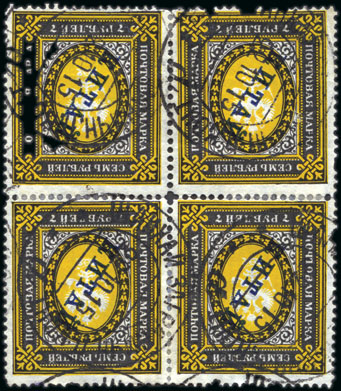
\includegraphics[width=.50\textwidth]{../russian-post-offices-in-china/10076.jpg}
\caption{
10076	SHANGHAI: Selection of stamps incl. T\&S type 5B (15), type 6A (9), 
type 6B (17), type 6 with unrecorded subtype Cyrillic "c" (on 1R), type 8A 
(45 incl. "KITAI" 3R50, 5R, 7R and 10R in blocks of four), with Arms, Romanov, 
"KITAI" and Chinese surcharged issues, incl. multiples, mixed condition, 
a difficult assembly.
\euro 500.00 
}  
\end{figure}


\begin{figure}[htbp]
\centering
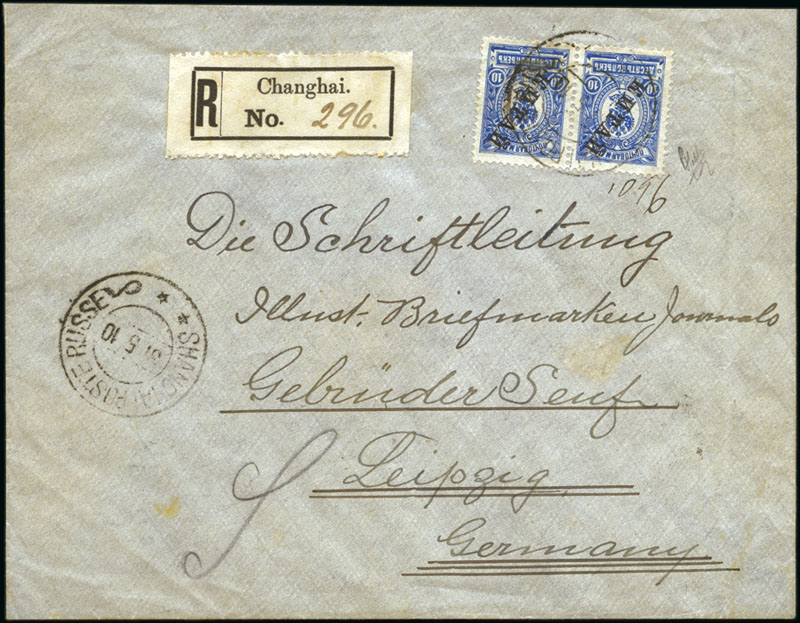
\includegraphics[width=.95\textwidth]{../russian-post-offices-in-china/10077.jpg}
\caption{
10077SHANGHAI: 1910 Cover sent registered to Germany with "KITAI" 10k pair 
tied by "SHANGHAI RUSSIAN POST b" 31.5.10 cds in French (Tchilinghirian type 6B), 
with unusual "Changhai" registered label in black adjacent, Leipzig bs, signed 
Holcombe
\euro 400.00 
}  
\end{figure}
 
\begin{figure}[htbp]
\centering
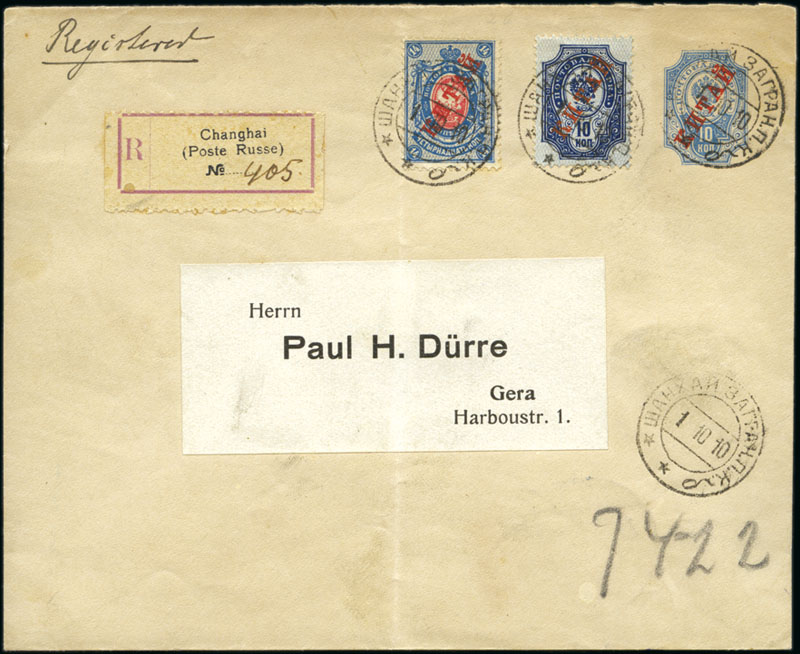
\includegraphics[width=.95\textwidth]{../russian-post-offices-in-china/10078.jpg}
\caption{
10078	SHANGHAI: 1910 "KITAI" 10k postal stationery envelope sent registered
to Germany, uprated with "KITAI" 10k and 14k, all cancelled by Shanghai 1.10.10 cds
(T\&S type 5B), with unusual "Changhai" reg'd label in French adjacent,
Gera bs, very fine and neat philatelic franking
\euro 200.00
}  
\end{figure} 

\begin{figure}[htbp]
\centering
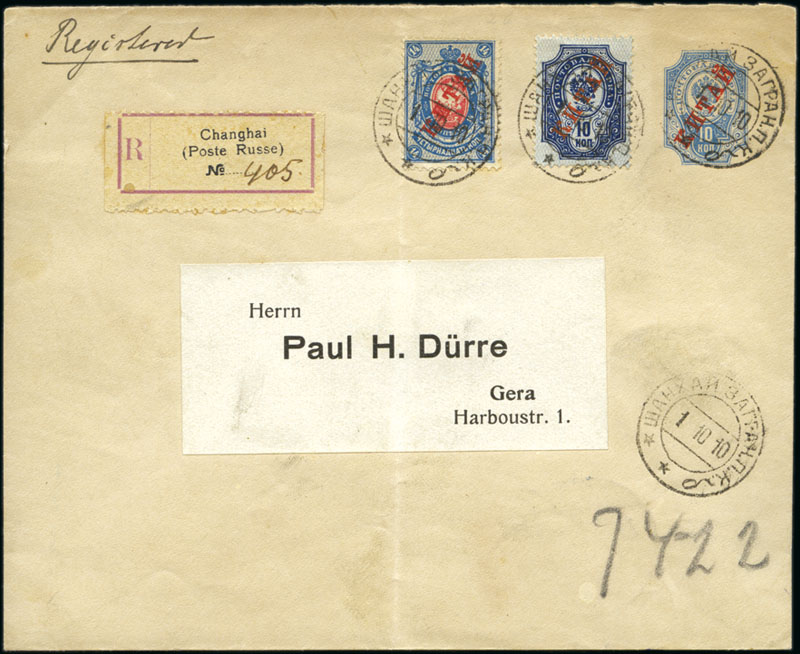
\includegraphics[width=.95\textwidth]{../russian-post-offices-in-china/10078.jpg}
\caption{
10078	SHANGHAI: 1910 "KITAI" 10k postal stationery envelope 
sent registered to Germany, uprated with "KITAI" 10k and 14k, 
all cancelled by Shanghai 1.10.10 cds (T\&S type 5B), with unusual 
"Changhai" reg'd label in French adjacent, Gera bs, very fine and neat 
philatelic franking
\euro 200.00
}  
\end{figure}


\begin{figure}[htbp]
\centering
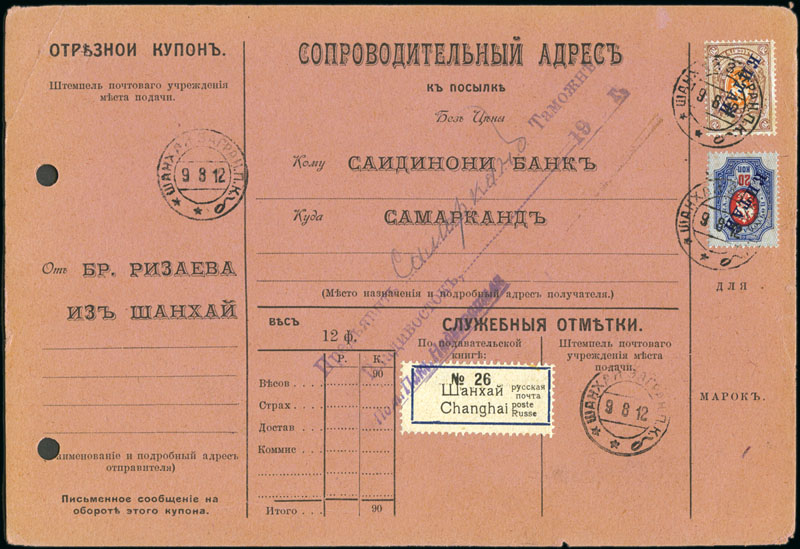
\includegraphics[width=.95\textwidth]{../russian-post-offices-in-china/10079.jpg}
\caption{
10079 SHANGHAI: 1912 Address card accompanying a parcel weighing 12 pounds 
to Samarkand (modern day Uzbekistan), with "KITAI" 20k and 70k paying the 
charges, tied by Shanghai 9.8.12 cds (T\&S type 5B), with insured label in 
Cyrillic and French adjacent tied by a three-line violet hs of Samarkand 
Customs, rare and unusual use.
\euro 300.00. 
}  
\end{figure}


          